\begin{document}
\begin{center}
{\LARGE\bfseries The AI-Level Index v2.0}\\[6pt]
{\large\bfseries A Tiered Standard on a Measured Instrument:\\[2pt] Evidence Tiers, a Specified Flash Bridge, Preregistered Reliability, Release-Day Operations,\\[2pt] and Six Studies of What the Scale Requires Before Its Numbers Mean Anything}\\[14pt]
{\large Chengshuai Yang$^{1,*}$ \quad Ting Xue$^{1}$}\\[5pt]
{\normalsize $^{1}$NextGen PlatformAI C Corp, USA}\\[4pt]
{\normalsize $^{*}$Correspondence: \href{mailto:spiritai@platformai.org}{spiritai@platformai.org}}\\[10pt]
{\small September 2026 --- version 2.0. Merges the v1.3 tiered standard (tiers, Flash bridge, trustworthiness pair, reliability rules, release-day operations) with the v2 instrument studies (recovery, resolution, anchoring, saturation, pricing, coverage). Supersedes both.}
\end{center}

\begin{abstract}
\noindent The AI-Level Index is the public model-comparison layer above Unified Intelligence Theory and AI-Level Bench: one number per frozen model, read through a published family of reference harnesses, on a scale whose levels are invariant by construction and whose delegation primitive prices a confident wrong answer below a declared inability. Two lines of work built it. The \emph{tiered standard} (v1.2--v1.3) separated five evidence tiers --- Flash, Core, Cert, Extended, Omega --- from the meaning of a level, specified a monotone bridge from a launch-day Flash score to the mature scale, wrote reliability as rules a program can apply, formalised trustworthiness as the pair of false-completion and false-rejection rates on solvable--blocked twin items, and derived release-day operations from the client as it exists. The \emph{instrument studies} (v2) asked what no index paper asks: whether the scale can carry the numbers it prints. On populations with known truth they found that the ordering is cheap and the interval is not; that the evidence needed to separate \emph{neighbouring} models grows as the square of the number ranked (measured exponent $2.4$: 128 witnesses to distinguish four models, 4096 for sixteen), so that a leaderboard must publish statistically indistinguishable bands rather than ranks; that free recalibration moves a cohort's already-published scores by $-0.53$ logits when a stronger cohort arrives while frozen anchors move them by $-0.01$, inside the $0.33$ standard error; that a fixed suite's bounded composite loses more than half its spread over three logits of frontier advance while witnesses refreshed within fixed levels hold it; that on $38.5\%$ of a competence-by-discrimination grid a success-only score prefers a bluffer and the delivered-outcome primitive prefers the system that declines; and that partial coverage is survivable while disjoint coverage is not. This version is the union. The tiers are the frame; the studies supply the numbers the frame's rules had to assume --- the minimum paired population for the bridge, the band rule that replaces rank robustness, the anchor policy behind frozen history, the coverage rule that says which rows may share a scale --- and the three rows the running instrument has produced are placed on the tier ladder as Flash-class evidence, with the latent fit published as the diagnostic the studies say it must be. Publication speed remains an operator competence disclosed beside the index and never inside it.
\end{abstract}

\noindent\textbf{Keywords:} AI-Level Index; evidence tiers; latent capability; item response theory; leaderboard resolution; anchoring and equating; benchmark saturation; false completion; false rejection; harness gain; release-day evaluation.

\tableofcontents
\bigskip

\section{Introduction}\label{sec:intro}

The AI-Level Index is the public model-comparison layer above Unified Intelligence Theory \citep{yang2026unified} and AI-Level Bench \citep{yang2026hilbench,yang2026hilbenchpaper}. Its measurement target is standardized agent-realizable intelligence: how much verified intelligence a frozen model realizes through a declared reference harness, and how much work can consequently be delegated to it under bounded human cognitive intervention. The categorical AI-Level and the full coordinate profile remain scientifically primary; the index compresses them into a number that supports ranking, trend analysis and communication.

Two problems shaped the two lines of work this version merges. The first is \emph{operational}: a scientifically careful index will be absent at the moment models are compared unless a fast, clearly qualified reading is available on release day. Versions 1.2 and 1.3 answered that with five evidence tiers on one ruler, a design principle restated here because everything below depends on it.

\begin{claimbox}{Design principle}
Publication speed is a core operational competence of AI-Level, but it is not an intelligence coordinate and is never added to the AI-Level Index score. A $C3$ claim means the same thing in Flash, Core, Cert, Extended and Omega; what changes is the amount and quality of evidence that may support it.
\end{claimbox}

The second problem is \emph{evidential}, and it is the one an index paper is not usually asked to face: whether the scale can carry the numbers it prints. Version 1.1 built a latent scale and reported that its own fit at two models was degenerate, without saying what would fix it. The v2 draft answered by measuring the estimator on populations with known truth --- how many models and witnesses recovery needs, what a rank costs, what anchors buy, what saturation does, what a bluff is worth, which coverage gaps are survivable. Several of those answers are numbers that v1.3's rules had to assume. This version puts them where they belong.

\subsection{Contributions of v2.0}
\begin{enumerate}[leftmargin=1.6em,itemsep=2pt]
\item \textbf{The tiered standard, kept} (\S\S\ref{sec:tiers}--\ref{sec:history}): five tiers on one ruler, the Flash bridge $g_F$, the trustworthiness pair, the reliability rules, frozen history and upgrades.
\item \textbf{The instrument measured} (\S\ref{sec:studies}): six studies on known-truth populations, with the tables and figures generated from the run.
\item \textbf{The rules re-derived from the studies}: the band rule replaces rank robustness (\S\ref{sec:reliability}, item 7); the bridge's minimum population is justified by the resolution law (\S\ref{sec:flash}); frozen history is an anchor policy with a measured effect (\S\ref{sec:history}); the coverage rule states which rows may share a scale (\S\ref{sec:reliability}, item 8); the proposition that no decline policy dominates gains its quantitative complement (\S\ref{sec:trust}).
\item \textbf{The measured baseline on the tier ladder} (\S\ref{sec:baseline}): the three rows the instrument has produced, labelled Flash-class, with the latent diagnostic and its dropped-item counts.
\item \textbf{Release-day operations as requirements} (\S\ref{sec:ops}) and \textbf{the cost of coverage} (\S\ref{sec:cost}), derived from the client as it exists, including the finding that usage is unrecorded.
\item \textbf{Validation program, tournament, tier-specific predictions, governance} (\S\S\ref{sec:validation}--\ref{sec:governance}), with three predictions already supported in simulation.
\end{enumerate}

\subsection{What it does not claim}
It does not claim the index is already more predictive than the incumbents: the tournament that would settle that is specified and has not been run. It does not claim the latent tier is ready to publish numbers: by its own criterion (\S\ref{sec:recovery}) it is not. It does not claim simulation substitutes for a broad measured population; simulation says what the population must contain.

\section{Relationship to Existing Capability Indices}\label{sec:related}

\textbf{Artificial Analysis Intelligence Index.} As of September 2026, v4.2 combines ten evaluations across four weighted categories \citep{aa2026index}, is independently run, reports uncertainty and keeps cost and speed separate from intelligence --- a product principle this index preserves. Its maintenance history is the argument for a different design: a saturated component was removed, new ones added, and private held-out weighting doubled. These are reasonable moves and they show that frontier discrimination on a fixed mixture requires recurring changes to the suite; \S\ref{sec:saturation} measures how fast.

\textbf{Epoch Capabilities Index.} ECI addresses saturation directly with an item-response scale over roughly sixty benchmarks, unbounded, with bootstrap uncertainty and fixed calibration points \citep{epoch2026eci}. This index does not compete with it by aggregating more benchmarks; its measurement object is different. Where ECI and this index share machinery --- a latent scale under measurement error --- the resolution law of \S\ref{sec:resolution} applies to both.

\begin{table}[!htbp]
\centering\small
\begin{tabularx}{\textwidth}{@{}p{3.1cm} Y Y Y@{}}
\toprule
 & Artificial Analysis & Epoch ECI & AI-Level Index \\
\midrule
Unit measured & a model through the evaluator's harness & a model's latent position across published benchmarks & a bare model through three \emph{published} harness rungs; the rung is part of the number \\
What a wrong answer costs & the missed point & the missed point & $\rho = 1$: a delivered wrong answer scores a full unit below a declared inability \\
Refusing an impossible task & not measured & not measured & measured on solvable--blocked twins (FCR and FRR) \\
Memory, learning, organization & not measured & not measured & $M0/I0$ by construction for a bare model and stated; $O0$ measured; the same items measure an agent \\
What a harness adds & not measured & not measured & Harness Gain and Harnessability on the rung curve \\
Items & fixed corpora & fixed corpora & seeded generators with computed keys; private split from a withheld salt whose hash is published \\
Ranks & ordered list & ordered list with intervals & bands: consecutive models whose intervals overlap are one group (\S\ref{sec:bands}) \\
Who runs a row & the index's authors & the index's authors & anyone, one command; certified when run independently on the private split \\
Speed & hours after launch, curated set & follows benchmark releases & Flash target six hours after \emph{evaluable} access; a KPI, not a score \\
\bottomrule
\end{tabularx}
\caption{Three indices, three measurement objects.}
\label{tab:related}
\end{table}

\textbf{Three questions.} AAI asks how strong a model is on a curated current suite; ECI asks where a model sits on a cross-benchmark latent scale; the AI-Level Index asks how much verified intelligence a model can realize as a standardized agent, and how much of it is real when the task cannot be done.

\section{Measurement Objects and What Must Not Be Double Counted}\label{sec:objects}

Unified Intelligence Theory uses five conceptual families, $C$, $I$, $O$, $DI$ and $SA$. The measured core is $[C, I, O, T, H, SA]$, with Delegation Intelligence derived from the task-difficulty and human-intervention surface at verified reliability $p$. Memory $M$ is certified on its own cumulative ladder and is a one-way prerequisite for higher $I$; it never promotes $I$. GUI perception is a diagnostic sub-ladder inside GUI-grounded cognition, a domain of $C$. Harness generation $HG$ is an engineering reference ladder --- $\mathrm{HG}_g = \mathrm{HG}_{g-1} + \Delta_g$, a strict mechanism superset, which is what makes a change in the curve attributable to one mechanism --- and $U$ is a conjunctive integration result, not a coordinate.

The singleton index therefore uses $C$, $I$, $DI$ and $SA$. A genuine organization is evaluated on a separate organizational leaderboard that adds $O$. Everything else --- $M$, $GP$, $HG$, $U$, cost, latency, throughput, publication speed --- is visible beside the index and never counted twice.

\begin{table}[!htbp]
\centering\small
\begin{tabularx}{\textwidth}{@{}l c Y@{}}
\toprule
Object & In the headline? & Role \\
\midrule
$C$ & yes & independent cognitive dimension \\
$I$ & yes & independent longitudinal individual dimension \\
$O$ & organizations only & N/A for singleton models; measured as an $O0$ floor and shown in metadata \\
$DI$ & yes & delegation construct derived from $T/H/p$ \\
$SA$ & yes & evidence-grounded self-awareness \\
$M$ & no & supporting cumulative prerequisite; reported separately to avoid double counting $I$ \\
$T, H, p$ & no & ordered axes and reliability used to construct $DI$ \\
$GP$, $C^{\mathrm{GUI}}$ & no & diagnostic and sub-domain evidence inside $C$ \\
$HG$ & no & reference-harness rung; architecture enables tests and earns nothing \\
$U$ & no & derived cumulative gate; adding it would be circular \\
cost, latency & no & deployment economics \\
publication speed & no & operator competence \\
\bottomrule
\end{tabularx}
\caption{What the headline may contain. For a singleton the $O0$ floor is measured and shown, so a reader is never left wondering whether it was omitted or unmeasured.}
\label{tab:objects}
\end{table}

\paragraph{Why four.} A bare model called through its API is $M0$ and $I0$ by construction and sits at $O0$; adding axes that cannot vary would add zeros to every row and dilute the aggregate without separating any two models. The same items measure an agent, for which memory, learning and organization become live, which is why HLIS and the level claim stay separate objects from the index. A choice about the product, not about intelligence, recorded as such.

\section{The Index}\label{sec:index}

\subsection{Evidence units and coordinate latent variables}
For frozen model $m$, harness condition $h$, coordinate $d$ and canonical evidence unit $i$,
\[
P(Y_{mdi} = 1) = \sigma\!\big[a_i(\theta_{md} - b_i)\big],
\]
with $\theta_{md}$ the model's capability on $d$, $b_i$ the calibrated witness difficulty and $a_i$ its discrimination; version 2.0 fits the one-parameter form and reports the two-parameter form as a robustness check. A unit may be a question, a delegation episode, a restart experiment or an entire campaign, once its measurement contract is frozen. Estimation is joint maximum likelihood with the origin at mean anchor difficulty, a mild ridge for identifiability, standard errors from the observed information, and one deliberate exclusion: a unit every model passes or every model fails is dropped \emph{and counted}, because it carries no information about who is stronger.

\subsection{Cumulative constraints}
No tier may reward level skipping. For every capability ladder the new gate and all lower-level retention must pass:
\[
A \models d_k \iff V_{d,k}(\text{new}) = 1 \;\wedge\; K_{d,<k} = 1, \qquad q^{*}_{d,k} = \min_{j \le k} q_{d,j}.
\]
$SA0$ is a baseline category; retention begins at $SA1$. $DI$ is cumulative as a frontier across lower $T$ bands at fixed $H$ and $p$; $T$ and $H$ are ordered axes of the item and the transcript, not capability ladders, and carry no retention.

\subsection{Singleton and organizational headline}
\[
G_S(m) = \sum_{d \in \{C, I, DI, SA\}} w_d\,\theta_{md}, \qquad
G_O(A) = \sum_{d \in \{C, I, O, DI, SA\}} w_d\,\theta_{Ad}, \qquad
\mathrm{AILI} = 100 + s\,G, \; s = 10 ,
\]
unbounded, so a frontier advance moves models up the scale rather than against a ceiling. Equal weights are a development convention only the tournament (\S\ref{sec:tournament}) may move. A certified singleton score requires all four coordinates measured under one index version; inapplicable dimensions are N/A, and applicable but unmeasured ones are never imputed as zero.

\subsection{Three objects, three questions}
\textbf{AI-Level / $U$}: what capability has been demonstrated --- a cumulative ordinal gate and profile. \textbf{HLIS}: how strong is this frozen pair --- a continuous pair score with bottleneck sensitivity. \textbf{AI-Level Index}: where does this base model sit on a common non-saturating scale --- a calibrated public scalar with an interval and a band.

\section{The Five Evidence and Publication Tiers}\label{sec:tiers}

Flash, Core, Cert, Extended and Omega are evidence-maturity tiers. They do not redefine any level. Flash optimizes time to first credible result; Core, breadth within a launch window; Cert, independent reproducibility and statistical confidence; Extended, long-horizon construct validity; Omega, evidence for repeated frontier expansion. A model may hold several historical tier records, each immutable and tied to a snapshot, harness version, witness generation and evaluator.

\begin{table}[!htbp]
\centering\small
\begin{tabularx}{\textwidth}{@{}l Y p{3.0cm} l Y@{}}
\toprule
Tier & Primary purpose & Publication target & Status & Unified ceiling by default \\
\midrule
AIL-Flash & launch-day preliminary signal & 2--6 h after independent evaluable access & preliminary & normally $U0$; no inferred longitudinal promotion \\
AIL-Core & broad preliminary profile & $<24$ h & preliminary & up to $U2$ when $I/M/SA/DI$ gates are actually run \\
AIL-Cert & independent official certification & days; $\le 7$ d for ordinary API models & certified & up to $U2$ by the base package \\
AIL-Extended & long-horizon advanced capabilities & multi-day to multi-week & certified-extended & $U3$--$U6$ where all canonical campaigns pass \\
AIL-Omega & open-ended frontier-expansion research & no fixed deadline & longitudinal research certification & $U\Om$ only with repeated bounded evidence and all retention \\
\bottomrule
\end{tabularx}
\caption{The five tiers. Targets are operator service objectives, not semantic definitions.}
\label{tab:tiers}
\end{table}

\section{AIL-Flash, Specified to the Call}\label{sec:flash}

Flash exists because model comparison is time-sensitive: a credible, clearly qualified signal within hours of a model becoming independently evaluable, measuring only constructs whose canonical evidence is fast to obtain, never pretending longitudinal capability has been established.

\subsection{Evidence package}
\begin{itemize}[itemsep=1pt]
\item \textbf{Cognition}: fast hidden or generated $C0$--$C4$ witnesses; bounded $C5$ only where a construct-valid secure generator exists.
\item \textbf{Delegation}: $T0$--$T3$ cells at predeclared $H$ budgets with the delivered-outcome primitive and false-completion accounting.
\item \textbf{Self-awareness}: grounded $SA1$--$SA2$ probes; no static self-report substitutes for runner truth.
\item \textbf{Individual and memory}: $I0$ and $M0$ by construction unless a genuine restart experiment is executed; Flash never infers $I1{+}$ from cognition.
\item \textbf{Harness}: $HG0$--$HG2$ for the rung curve and Harness Gain.
\item \textbf{Metadata}: per-call usage, cost, latency, tool calls, FCR, FRR, held-back rate, evaluator, snapshot, resource envelope, access route, $t_{\text{access}}$.
\end{itemize}

\subsection{Per-release seed commitment}
Flash uses public generators with fresh hidden seeds. So that a launch-day row cannot be accused of seed selection after the fact, the evaluator publishes $\mathrm{SHA\text{-}256}(\text{salt}_r)$ for release $r$ \emph{before} the first call, derives the seeds by the benchmark's HMAC rule, and reveals $\text{salt}_r$ with the row. The cost is one hash.

\subsection{The Flash score and the bridge to the mature scale}
Flash lacks the Individual evidence the four-coordinate index requires, so it must not silently renormalise $C$, $DI$ and $SA$ and call the result an AILI. Its public number is the \textbf{AIL-Flash Score} $S_{\mathrm{Flash}} \in [0, 100]$, a bounded composite whose formula is versioned; the running instrument's composite (\S\ref{sec:baseline}) is one such formula.

\begin{claimbox}{The bridge $g_F$}
\begin{enumerate}[leftmargin=1.4em,itemsep=2pt]
\item \textbf{Form.} $g_F$ is a monotone non-decreasing map fitted by isotonic regression of Cert-tier AILI on $S_{\mathrm{Flash}}$ over models holding both rows on compatible versions. Monotonicity is the only shape assumption.
\item \textbf{Minimum population.} $g_F$ is not fitted, and no Flash row shows an AILI-scale value, until $N_{\text{pair}} \ge 20$ models span at least four of the five Cert quintiles present. \emph{Why twenty:} by the resolution law (\S\ref{sec:resolution}) twenty models on a few hundred witnesses give a good ordering and almost no adjacent separation, so the bridge is fitted on a population that can be ordered but not finely resolved; fewer models would make the isotonic fit a step function through noise. Below the minimum, Flash rows display $S_{\mathrm{Flash}}$ only, labelled preliminary.
\item \textbf{Equating error.} The leave-one-out RMS difference between $g_F^{(-m)}(S_m)$ and $\mathrm{AILI}_m^{\mathrm{Cert}}$ is the equating error $e_F$; every bridged interval is the Flash interval widened by $\pm 1.96\,e_F$, both components shown.
\item \textbf{Freeze.} $g_F$ and $e_F$ are frozen per index version; adding paired rows produces a new minor version, never a silent refit.
\item \textbf{Falsification.} If the running RMSE over the last ten new pairs exceeds $1.5\,e_F$, bridged display is suspended for the version and the failure is published.
\end{enumerate}
\end{claimbox}

\subsection{Reporting string}
\begin{center}\small
\texttt{AIL-Flash S\_Flash [preliminary] | Cx | T/H@p | SAy | I: pending | M: pending | FCR | FRR | Gain}
\end{center}
Until $g_F$ is frozen the leading number is $S_{\mathrm{Flash}}$ in its own units; after freezing it may be followed by ``$\approx\mathrm{AILI}\ \hat y\,[\ell, u]$ via $g_F$/Index-2.x''. An AILI-scale value never appears in the Flash position before the bridge exists.

\section{Trustworthiness: False Completion and False Rejection}\label{sec:trust}

The delivered-outcome primitive prices a delegation cell as
\[
S_{\mathrm{net}} = P(\text{delivered} \wedge \text{verifier pass}) \;-\; \rho \cdot P(\text{false completion}),
\]
with $\rho = 1$ in every tier: a delivered wrong answer costs a full unit, a declared inability costs nothing beyond the missed point. The obvious objection is that a model could win by declining everything.

\begin{definition}[Twin item]
A twin item is a pair $(x^{\circ}, x^{\bullet})$ generated from one seed such that $x^{\circ}$ is solvable under the declared contract and $x^{\bullet}$ differs only in a witness-checkable property that makes it unsatisfiable. The verifier knows which is which; the model is told neither.
\end{definition}

\begin{definition}[FCR and FRR]
Over the twin population, the \textbf{false-completion rate} is the fraction of blocked twins on which a deliverable was produced and passed no verifier; the \textbf{false-rejection rate} is the fraction of solvable twins on which the model declared inability; the \textbf{held-back rate} is the fraction of all items declined.
\end{definition}

\begin{proposition}
Under $\rho = 1$ with twin items, no fixed decline policy dominates. Declining every item sets $\mathrm{FCR} = 0$ and $\mathrm{FRR} = 1$, forfeiting the delivery term on every solvable twin; delivering on every item sets $\mathrm{FRR} = 0$ and pays $\rho$ on every blocked twin. The score is maximised only by discriminating the two, which is the construct.
\end{proposition}

\paragraph{The quantitative complement.} The proposition says no policy dominates; \S\ref{sec:bluff} measures how often the choice of primitive changes the answer. Across a grid of competence and discrimination, on $38.5\%$ of cells a success-only score ranks a bluffing system at or above one that declines while $S_{\mathrm{net}}$ reverses the order --- more than a third of the plausible parameter space. And $\rho$ is not a taste: if a wrong delivery costs the delegator $c_{\mathrm{wrong}}$ and a held-back task costs $c_{\mathrm{redo}}$, expected cost is $c_{\mathrm{wrong}}P(\text{FC}) + c_{\mathrm{redo}}P(\text{held back})$, and $S_{\mathrm{net}}$ is its linear proxy at $\rho = c_{\mathrm{wrong}}/c_{\mathrm{redo}}$. The ratified $\rho = 1$ says an undetected wrong answer costs about what redoing the task costs; where it costs more, the constant changes, and with it the version.

\paragraph{Why the pair stands beside the headline.} Neither incumbent measures either rate, and neither can add them without items designed to be unsatisfiable and a scoring rule in which a wrong delivery costs more than an admission. Both exist here. The pair answers the question users ask most and no leaderboard answers, and it is the component least exposed to saturation: a frontier that no longer bluffs on the hardest blocked witnesses is a finding, not a failure of the instrument.

\section{Preregistered Reliability, Stopping and Publication Rules}\label{sec:reliability}

These are the defaults a conforming implementation uses unless a registered protocol replaces them. Rules 7 and 8 are new in v2.0 and come from \S\ref{sec:studies}.

\begin{enumerate}[leftmargin=1.6em,itemsep=2pt]
\item \textbf{Rates.} FCR, FRR, held-back rate and every per-cell pass rate carry a Wilson 95\% interval; exact binomial where $n < 10$.
\item \textbf{Latent coordinates.} $\theta_{md}$ carries a bootstrap or posterior 95\% interval; the interval is published with the point, never separately.
\item \textbf{Gating bands.} Any cell used to decide a level claim holds at least $n_{\min} = 12$ episodes: the bare DeepSeek row read 35.2 on both the public and the private split once the gating band carried twelve, and a pair's level moved from $U0$ to $U1$ on the same extension.
\item \textbf{Sequential stopping.} Sample until the interval half-width is $\le \delta = 0.10$ or $n = n_{\max} = 48$; report which stopped the run. Fixed before the first episode.
\item \textbf{No imputation.} An applicable but unmeasured coordinate blocks a full headline for the tier; the row shows the coordinate as \emph{pending}, never as zero, and the rest is not renormalised into a full-looking scalar.
\item \textbf{Variance gate.} Items with no between-model variance are dropped from the fit and \emph{counted} per coordinate. A fit in which a coordinate retains zero items is a diagnostic, never a row.
\item \textbf{Bands, not ranks} (replaces rank robustness). Models are ordered by $\mathrm{AILI}$ and consecutive models whose 95\% intervals overlap are published as one band; no order is reported inside a band. This is the consequence of the resolution law (\S\ref{sec:resolution}): the evidence required to separate neighbours grows as the square of the number ranked, so a rank inside a band is a claim no feasible evidence base supports. Weight perturbation ($\pm 0.10$ on the simplex) and seed resampling are still run before ratification, and a top-five order that changes under them is reported as one band.
\item \textbf{Shared anchors} (coverage). Every published row shares a minimum anchor witness set with every other row on the same scale. Partial coverage with shared anchors is survivable; disjoint coverage is not (\S\ref{sec:coverage}). A row that shares nothing with the rows above it is not placed on the scale.
\end{enumerate}

\section{AIL-Core and AIL-Cert}\label{sec:corecert}

\textbf{Core} is the first tier that estimates the full singleton vector $[C, I, DI, SA]$ rather than a launch-day proxy, with a publication target under 24 hours: a broader $C0$--$C5$ battery, $M0$--$M3$ with genuine process restart and provenance tests, $I0$--$I2$ including restart continuity and experienced-versus-ablated transfer under a frozen learning mechanism, systematic $T0$--$T3$ across $H0/H1$ and where available $H2$, $SA1$--$SA3$ when the fault-injection protocol completes, $O0$--$O2$ for genuine organizations, $HG0$--$HG3$ paired on the same seeds. Core may issue a provisional AILI with the Core badge and a wider interval.

\textbf{Cert} is the normative public certification tier, defined not by being slow but by independence, private or permanently committed evidence, calibrated difficulty, explicit uncertainty and complete coordinate coverage: an evaluator independent of the builder; the three evidence surfaces (public reference forms, permanent private anchors, fresh hidden witnesses); preregistered rules per \S\ref{sec:reliability}; lower-level retention re-run for every cumulative claim; all four singleton coordinates measured, $O$ for organizations, $M$ separately; no renormalisation over unmeasured coordinates; and an immutable record. Its normal Unified ceiling is $U2$; a $U3{+}$ headline requires Extended.

\section{AIL-Extended and AIL-Omega}\label{sec:extomega}

\textbf{Extended} measures constructs whose meaning includes time: $C6$ and high-difficulty $C5$, $M4$--$M5$, $I3$--$I5$ self-improvement and meta-campaigns, $O3$--$O5$, $T4$--$T6$ under low $H$, $SA4$--$SA6$, $HG4$--$HG6$ conformance and $U3$--$U6$. Results stay on the same scale; added evidence changes coordinate estimates, narrows intervals and may support higher categorical claims. Publication time is set by the construct.

\textbf{Omega} is the research track for open-ended claims. Finite experiments cannot prove infinity; Omega certification means repeated, bounded, independently verified evidence that the system expands its own reachable frontier across cycles, under causal ablation, over several domain families, with persistent lineage and governance and all lower retention. Its record names horizon, validated cycles and domains: $\mathrm{AILI} \mid U\Om(H, N, D) \mid [C\Om, I\Om, DI(T\Om/H0), SA\Om] \mid M\Om$.

\section{One Scale, Frozen History, Upgrades}\label{sec:history}

Evidence accumulates; it is not discarded. Flash items are a strict subset or construct-equivalent precursor of later evidence; each tier adds to the set. Coordinate estimation uses the same frozen anchors and only the evidence set changes:
\[
\theta^{(\tau)}_{md} = \text{estimate}(\theta_{md} \mid E_\tau, \text{anchors}, \text{version}), \qquad
\mathrm{AILI}_\tau = 100 + s \sum_d w_d\,\theta^{(\tau)}_{md}.
\]
A later tier never overwrites an earlier result; it creates a new immutable record linked to the same snapshot. Witness renewal changes no level and rewrites no score; a semantic change opens a new major standard.

\paragraph{Frozen history is an anchor policy, with a measured effect.} ``Never recomputed'' is only a promise unless the estimator has a fixed origin. \S\ref{sec:anchors} measures what happens without one: when a stronger cohort arrives and everything is recalibrated together, the earlier cohort's published scores fall by $0.53$ logits --- five index points --- for no reason connected to their capability; with anchors frozen, the movement is $0.01$ logits, inside the standard error. Hence the two-track rule: a \emph{frozen historical} index that is never recomputed under one version, and a \emph{current-fit} view published separately and labelled a diagnostic.

\section{Six Studies of the Instrument}\label{sec:studies}

Everything above is design. What follows is measurement on populations where the truth is known by construction, so the estimator can be scored against it. The six studies are in \texttt{hilbench/index\_sim.py}, run by one command, and the tables and figures below are generated from the run they write; a test asserts that the vectorized estimator used here agrees with the package's canonical one on a shared case, so speed did not buy a different answer.

\subsection{Recovery: what the estimator needs}\label{sec:recovery}

Simulate $M$ models with abilities from a unit normal and $K$ witnesses with difficulties from $\mathcal N(0, 1.2)$, generate responses under the model, fit, compare with truth. Table~\ref{tab:sample} reports, per cell, the rank correlation, the share of \emph{adjacent} pairs whose 95\% intervals do not overlap, and the median standard error in logits (one logit is ten index points).

\begin{table}[!htbp]\centering\small
\begin{tabular}{@{}lcccc@{}}\toprule
$M$ & $K=40$ & $K=80$ & $K=160$ & $K=320$ \\ \midrule
2 & 1.00 / 1.00 / 0.61 & 1.00 / 1.00 / 0.41 & 1.00 / 1.00 / 0.31 & 1.00 / 1.00 / 0.19 \\
3 & 1.00 / 0.00 / 0.47 & 1.00 / 0.50 / 0.35 & 1.00 / 0.50 / 0.24 & 1.00 / 0.50 / 0.16 \\
5 & 0.90 / 0.00 / 0.44 & 0.90 / 0.25 / 0.30 & 1.00 / 0.50 / 0.21 & 1.00 / 0.50 / 0.15 \\
8 & 0.83 / 0.00 / 0.40 & 0.93 / 0.00 / 0.29 & 0.95 / 0.14 / 0.20 & 0.98 / 0.29 / 0.14 \\
12 & 0.92 / 0.00 / 0.39 & 0.94 / 0.00 / 0.28 & 0.97 / 0.09 / 0.20 & 0.98 / 0.14 / 0.14 \\
20 & 0.94 / 0.00 / 0.39 & 0.96 / 0.00 / 0.27 & 0.97 / 0.00 / 0.19 & 0.99 / 0.11 / 0.13 \\
40 & 0.93 / 0.00 / 0.38 & 0.96 / 0.00 / 0.27 & 0.98 / 0.00 / 0.19 & 0.99 / 0.03 / 0.13 \\
\bottomrule\end{tabular}
\caption{Recovery against known truth: Spearman / share of adjacent pairs separated at 95\% / median standard error, at $M$ models and $K$ witnesses, median over 30 replications. Spearman is uninformative below about eight models --- with two or three, any estimator orders them almost surely --- which is why the middle number matters more.}
\label{tab:sample}
\end{table}

Two readings. \emph{The ordering is cheap and the interval is not}: rank correlation passes $0.95$ at 160 witnesses and stays there, while the standard error falls only as $1/\sqrt K$, from $0.39$ logits at $K = 40$ to $0.13$ at $K = 320$ --- from $\pm 7.6$ to $\pm 2.6$ index points. An index published from a small evidence base can say who is ahead and cannot say by how much. And, less comfortably, \emph{adjacent separation falls as the population grows}: at four models and 320 witnesses half of neighbouring pairs are distinguishable; at forty, three per cent are. Nothing is wrong with the estimator; the gaps between neighbours shrink faster than the errors do.

\subsection{The resolution law: what a rank costs}\label{sec:resolution}

For $M$ abilities from a unit normal the typical gap between neighbours near the middle is about $\sqrt{2\pi}/M \approx 2.5/M$. Separating two estimates at 95\% requires their gap to exceed $1.96\sqrt2\,\mathrm{SE} \approx 2.77\,\mathrm{SE}$, so
\[
\mathrm{SE} \lesssim \frac{0.9}{M}, \qquad \text{and since } \mathrm{SE} \approx \frac{2}{\sqrt K}, \qquad K \gtrsim 5M^2 .
\]
Doubling the number of models a leaderboard wants to \emph{rank} quadruples the evidence each must supply. Figure~\ref{fig:resolution} scans for the smallest $K$ at which half of adjacent pairs separate: 128 witnesses for four models, 512 for six, 1024 for eight, 2048 for twelve, 4096 for sixteen; log--log slope $2.4$. The exponent exceeds the idealized $2$ because difficulties are spread rather than matched to the population and uninformative items are dropped.

\begin{figure}[!htbp]\centering
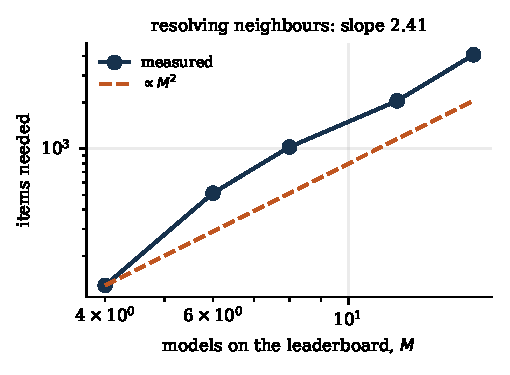
\includegraphics{fig_resolution.pdf}
\caption{Items needed before half of adjacent models separate at 95\%, against the number of models ranked, with the $M^2$ reference. Ranking is quadratically more expensive than scoring.}
\label{fig:resolution}
\end{figure}

This is a property of ranking under measurement error and applies to every leaderboard, including the incumbents. An index that prints a hundred ordered rows is making a claim about resolution that no feasible evidence base supports; the response is not more items but to stop printing the rank.

\subsection{Bands, not ranks}\label{sec:bands}
Hence rule 7 of \S\ref{sec:reliability}: models are ordered by $\mathrm{AILI}$, consecutive models whose intervals overlap are one band, and no order is reported inside it (\texttt{index\_sim.bands}). A band boundary is a claim the evidence supports; a rank inside a band is not. It costs nothing that was real, removes the part of a leaderboard most often over-read, and makes uncertainty visible in the artefact people look at rather than in a column they skip.

\subsection{Anchors, and whether last year's score still means anything}\label{sec:anchors}

Simulate eight models on an anchor set; add eight stronger models measured on the anchors plus fresh witnesses whose difficulty tracks the new frontier; ask what happened to the first cohort's published scores.

\begin{table}[!htbp]\centering\small
\begin{tabular}{@{}lcc@{}}
\toprule
Calibration policy & Systematic drift (logits) & Absolute drift (logits) \\
\midrule
Free recalibration over all data & $-0.53$ & $0.57$ \\
Frozen anchors carry the scale & $-0.01$ & $0.36$ \\
\midrule
\multicolumn{3}{@{}l}{\emph{measurement noise for reference: median SE $= 0.33$ logits}} \\
\bottomrule
\end{tabular}
\caption{What adding a stronger cohort does to the previous cohort's published scores, median over 30 replications. Absolute drift mixes noise with bias; the signed drift is the bias.}
\label{tab:equating}
\end{table}

Free recalibration is the natural thing to do and it silently rewrites history: the origin follows the mean difficulty of whatever items are in the pool, so harder items for a stronger cohort push everyone already on the board downwards. Frozen anchors remove the bias entirely. This is the measurement behind \S\ref{sec:history}.

\subsection{Saturation: a fixed suite stops measuring}\label{sec:saturation}

Let the frontier advance $0.6$ logits a year for five years and compare a suite fixed at its year-zero difficulties with one whose witnesses are refreshed within fixed levels so difficulty tracks the population --- ``saturation motivates harder witnesses, not a redefined level'', implemented.

\begin{table}[!htbp]\centering\small
\begin{tabular}{@{}lcccccc@{}}\toprule Frontier & \multicolumn{3}{c}{bounded composite} & \multicolumn{2}{c}{separation} & at ceiling \\ \cmidrule(lr){2-4}\cmidrule(lr){5-6}
(logits) & mean, fixed & spread, fixed & spread, refreshed & fixed & refreshed & fixed \\ \midrule
0.0 & 0.52 & 0.162 & 0.176 & 0.96 & 0.96 & 0.00 \\
0.6 & 0.58 & 0.167 & 0.174 & 0.97 & 0.96 & 0.00 \\
1.2 & 0.70 & 0.147 & 0.168 & 0.95 & 0.96 & 0.00 \\
1.8 & 0.76 & 0.133 & 0.181 & 0.95 & 0.97 & 0.00 \\
2.4 & 0.86 & 0.085 & 0.166 & 0.92 & 0.96 & 0.17 \\
3.0 & 0.91 & 0.074 & 0.184 & 0.87 & 0.97 & 0.33 \\
\bottomrule\end{tabular}
\caption{Three logits of frontier advance. The fixed suite's bounded composite rises from $0.52$ to $0.91$ and its spread collapses from $0.162$ to $0.074$, with a third of models at its ceiling; the refreshed suite holds spread and separation.}
\label{tab:saturation}
\end{table}

\begin{figure}[!htbp]\centering
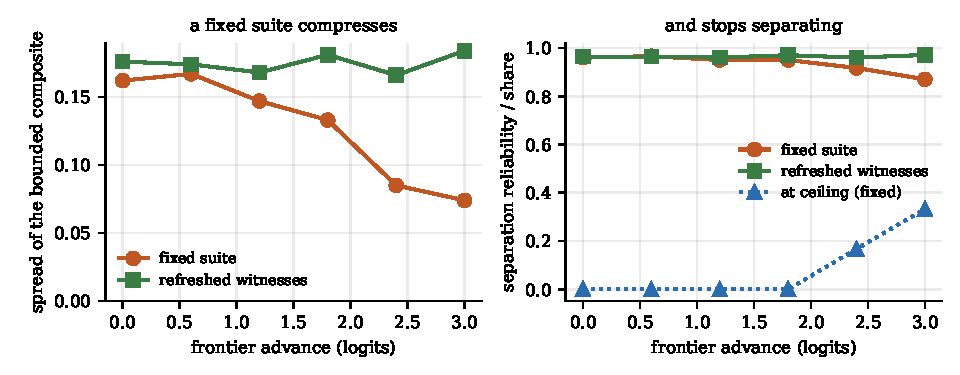
\includegraphics{fig_saturation.pdf}
\caption{Left: the spread of a bounded composite --- the AAI-shaped quantity --- against frontier advance. Right: separation reliability, and the share of models at the fixed suite's ceiling.}
\label{fig:saturation}
\end{figure}

The bounded composite degrades fast: more than half its spread is gone after three logits, which is what forces a maintained index to swap components. The latent fit on the same fixed suite degrades more gracefully ($0.96 \to 0.87$) because it estimates ability rather than averaging scores --- an argument for ECI's approach over a weighted mean --- but it degrades, and a third of models at the ceiling of every item is a limit no estimator sees past. The benchmark has run this for real: two models a tenfold cost apart both scored $90.0$ on the Core, the instrument's ceiling; four harder witnesses admitted after a program verified each satisfied its level's law separated them by 46 points, and no level changed meaning.

\subsection{Pricing a bluff}\label{sec:bluff}

Two systems of equal competence $q$: one attempts everything; one declines what it judges it cannot do, with some skill at telling its failures from its successes and occasional false rejection. Across a grid of competence and discrimination, on $38.5\%$ of cells a success-only score ranks the bluffer at or above the decliner while $S_{\mathrm{net}}$ reverses the order. That is the region where the two indices would give a buyer opposite advice, and it is more than a third of the plausible space. The cost identity of \S\ref{sec:trust} is what makes $\rho$ a measurable quantity rather than a preference.

\subsection{Coverage: linking needs common items, not complete ones}\label{sec:coverage}

\begin{table}[!htbp]\centering\small
\begin{tabular}{@{}lccc@{}}\toprule Coverage & Spearman & median SE & SE, partial models \\ \midrule
complete & 0.965 & 0.19 & 0.19 \\
missing at random, 40% & 0.951 & 0.26 & 0.26 \\
blocked by difficulty, items shared & 0.965 & 0.24 & 0.28 \\
disjoint: the halves share no item & 0.853 & 0.29 & 0.30 \\
\bottomrule\end{tabular}
\caption{Ordering recovery and interval width under four coverage regimes, twelve models and 160 witnesses. ``SE, partial models'' is the interval on the models that skipped part of the suite.}
\label{tab:coverage}
\end{table}

The result corrected the authors' own intuition. Blocked coverage --- half the models running only the easy half --- costs almost nothing in ordering ($0.965$ against $0.965$ complete), because the hard witnesses are still answered by the other half and carry the scale; the models that skipped are placed with a wider interval ($0.28$ against $0.19$), which is the correct behaviour. What breaks the scale is \emph{disjoint} coverage: ordering falls to $0.85$ and the two halves are no longer on one scale. Hence rule 8 of \S\ref{sec:reliability}, and the design consequence for the tiers: Flash's items must be a subset of Cert's precisely so that every tier shares anchors with every other.

\section{Where the Instrument Stands: The Measured Baseline}\label{sec:baseline}

\subsection{The composite that runs today}
The command \texttt{hilbench index} computes
\[
S_{\mathrm{rapid}} = 0.55\cdot\mathrm{AUC}_{HG0..HG2} + 0.35\cdot\mathrm{Ceiling} + 0.10\cdot\mathrm{Harnessability} \in [0, 100],
\]
over three seeds per family and both Core-H seeds, about 100--150 calls, with $\rho = 1$, on the public split or with the withheld salt on the private one. In tier vocabulary this is an \textbf{AIL-Flash Score}: it reads $C$, $DI$ and $SA$ quickly through three published harness rungs, sets $I0$ and $M0$ by construction, measures $O0$ as a floor, and has never executed a restart or learning experiment. It is a Flash-class instrument and not a Core one.

\begin{table}[!htbp]\centering\footnotesize
\begin{tabular}{@{}p{3.2cm}p{2.4cm}cccc c>{\raggedright\arraybackslash}p{1.5cm}@{}}\toprule Model & Split & Index & HG0/HG1/HG2 & Gain & FCR & Decl. & Profile \\ \midrule
DeepSeek \texttt{deepseek-chat} & public, 3 seeds/family & \textbf{32.3} & 35.9/35.9/35.9 & 0.0 & 0.00 & 0.06 & C3, SA1, T1 \\
DeepSeek \texttt{deepseek-chat} & private, 4 salt-derived seeds & \textbf{35.2} & 31.3/39.5/39.2 & 8.2 & 0.04 & 0.04 & C3, SA1, T1 \\
Qwen 3.8 27B \texttt{qwen3.8:27b} & public, 3 seeds/family & \textbf{30.3} & 26.1/34.9/31.3 & 8.8 & 0.08 & 0.10 & C3, SA1, T0 \\
\bottomrule\end{tabular}
\caption{Every row the instrument has produced, as Flash-class evidence. All were run by the instrument's author, who built neither model; under \S\ref{sec:corecert} none is certified. The smaller model bluffs three times bare and gains 8.8 points from a harness that catches part of it; the larger bluffs nowhere on the public split and gains nothing there. That a harness helps the model that fails catchably is the first prediction of \S\ref{sec:predictions}, on two rows. By rule 7 the three rows are one band.}
\label{tab:baseline}
\end{table}

\subsection{The latent fit at $N = 2$, published as a diagnostic}
Fitting the unbounded scale over these rows gives $\theta_H = +3.10$ and $-3.10$ with standard errors of 3.88, and a latent index of 131.0 with a 95\% interval of $[54.9, 207.1]$ for the higher model --- an interval wider than the scale. Of the cognition items, 42 of 42 showed no between-model variance and were dropped; of the delegation items, 72 of 78; of the self-awareness items, 14 of 18; coordinate $C$ retained zero items and the fit fell back to $DI$ and $SA$. This is what \S\ref{sec:recovery} predicts for a two-model population: the ordering is trivially right and the interval is meaningless. The number is a diagnostic and not a row.

\subsection{What the baseline tells the standard}
The tier the instrument reaches is Flash, so the first engineering target is Core: a restart experiment executable inside a launch window. The bridge $g_F$ cannot be fitted for want of Cert rows. And the cost claim of ``cents per row'' inherited from v1.1 rests on a call count, not on tokens; the runner records no usage, and \S\ref{sec:ops} makes the accounting mandatory.

\section{Release-Day Operations as Requirements}\label{sec:ops}

\subsection{The access timestamp, operationally}
\begin{definition}[$t_{\text{access}}$]
The first wall-clock time at which an evaluator in the AI-Level network completes an authenticated call to the model under the required contract --- a tool-enabled chat completion returning a well-formed response --- and logs the request and response hashes. Provider announcements, waitlists and inaccessible previews do not start the clock.
\end{definition}
\begin{align*}
\mathrm{TTFR} &= t_{\mathrm{Flash}} - t_{\text{access}}, \qquad \mathrm{TTCR} = t_{\mathrm{Cert}} - t_{\text{access}},\\
\mathrm{Coverage}_{7d} &= \#\{\text{major evaluable releases with a} \ge \text{Core row within 7 d}\} \,/\, \#\{\text{major evaluable releases}\}.
\end{align*}
All three are operator KPIs on the coverage dashboard and never enter any score.

\subsection{Access routes}
The network must not depend on one person holding every provider account. Three routes share the same server-side tasks and verifiers: \textbf{direct} (the evaluator's own accounts, including aggregator endpoints that list new models within hours, which is how day-one coverage of the long tail is obtained); \textbf{vendor-provided} (temporary or embargoed endpoints, with the evaluator controlling tasks, seeds, scoring and publication, official only if independence is preserved); and \textbf{independent verified endpoint} (an approved external lab, the server retaining hidden forms and the verifier). A self-run submission is never silently upgraded to Cert.

\subsection{Client requirements derived from the instrument}
Each item names a property of the current client and the requirement that replaces it.
\begin{enumerate}[leftmargin=1.6em,itemsep=1pt]
\item \textbf{Usage accounting.} The client records no token usage. \emph{Requirement:} capture the provider's usage block per call, total it per row, publish cost from posted prices at run time with the price sheet hashed into the record.
\item \textbf{Retry with backoff.} One request per call, no retry; a rate-limited provider yields a failed row in the week limits bite hardest. \emph{Requirement:} exponential backoff with jitter on 429 and 5xx, a bounded retry count, and a record distinction between an item the model failed and one the provider failed to serve.
\item \textbf{Parameter negotiation.} Temperature zero is sent unconditionally; several reasoning models reject it. \emph{Requirement:} a per-provider capability probe with the negotiated parameters recorded.
\item \textbf{Adapters.} Two API shapes are supported. \emph{Requirement:} an adapter per native interface or routing through an aggregator, recorded as the access route.
\item \textbf{Snapshot pinning.} Providers mutate a model behind a stable name. \emph{Requirement:} record the exact snapshot and run date; a silent change is a new row, never an update.
\item \textbf{Spend guard.} An unattended loop stops at a stated budget per row and per day.
\item \textbf{Seed commitment.} Publish the release salt hash before the first call.
\item \textbf{The watcher.} Poll the network's model lists, diff against rows held, run Flash unattended on anything new. This is the single mechanism that makes coverage a property of the system rather than of whoever is awake.
\end{enumerate}

\subsection{A public service level}
Once the watcher and the retry layer exist, the operator publishes a service objective it can meet --- a Flash row within 24 hours of $t_{\text{access}}$ for any model reachable by a direct route --- and reports attainment. Speed that can be guaranteed is worth more than speed that depends on a vendor's goodwill.

\section{The Cost of Coverage}\label{sec:cost}

No one can state the cost per row today, including the authors, because the runner records no usage. The sizing below is an estimate with its assumptions named.

\begin{table}[!htbp]
\centering\small
\begin{tabularx}{\textwidth}{@{}l c c Y@{}}
\toprule
Model class & Assumed tokens per row & Rough cost per row & Assumption \\
\midrule
small or open weights & $\sim$0.6M & a few cents & 150 calls at $\sim$3k input and $\sim$1k output tokens; low posted prices \\
typical frontier, no heavy reasoning & $\sim$0.6M & a few dollars & same token profile; mid-range prices \\
heavy reasoning & several million & tens of dollars & reasoning tokens dominate and are billed as output \\
\bottomrule
\end{tabularx}
\caption{Cost per Flash row by model class. Assumptions, not measurements.}
\label{tab:cost}
\end{table}

At thirty new or updated models a month the monthly spend is plausibly in the low hundreds of dollars, rising sharply if reasoning models dominate. The dominant uncertainty is reasoning-token consumption, which is exactly what the missing instrumentation would settle. And the resolution law adds a second line to the budget: separating neighbours on a board of $M$ models costs of order $M^2$ witnesses per model, so a leaderboard that wants fine ranks is buying evidence quadratically. Bands are cheaper than ranks because they are honest about that.

\section{Reporting, Leaderboards, Public Interpretation}\label{sec:public}

A single number is the entry point, not the result. Every row displays its tier, trust status and \emph{band}, so that speed cannot masquerade as certification and a rank cannot masquerade as resolution. Required fields per row: tier; trust status; headline ($S_{\mathrm{Flash}}$ or AILI with interval and version); band; highest certified $U$ with pending shown; profile $[C, I, T/H, SA]$ or $[C, I, O, T/H, SA]$; $M$ separately; delegation frontiers; reliability (interval, sample count, stopping rule); trustworthiness (FCR, FRR, held-back rate); harness (rung curve, Harness Gain); economics (cost, tokens, calls, latency); coverage metadata (snapshot, evaluator, access route, TTFR/TTCR, witness generation, resource envelope).

\paragraph{Compact strings.}
\begin{center}\footnotesize
\begin{tabularx}{\textwidth}{@{}l >{\raggedright\arraybackslash\ttfamily}X@{}}
Flash & AIL-Flash 32.3 [preliminary] | band 1 of 1 | C3 | T1/H0@.80 | SA1 | I pending | M pending | FCR .00 | FRR .06 \\
Core & AILI 174 [Core] | band 2 | U2? pending Cert | [C5,I2,T3/H1,SA3] | M3 \\
Cert & AILI 176 [Certified] | band 2 | U2 | [C5,I2,T3/H1,SA3] | M3 \\
Extended & AILI 189 [Extended] | band 1 | U4 | [C6,I4,T4/H1,SA4] | M4 \\
Omega & AILI 205 [Omega] | band 1 | U$\Om$(H=12mo,N=5,D=4) | [C$\Om$,I$\Om$,T$\Om$/H0,SA$\Om$] | M$\Om$ \\
\end{tabularx}
\end{center}
\noindent The Flash example is a real row in $S_{\mathrm{Flash}}$ units; the others are illustrative, and no such row exists.

\section{Validation Program}\label{sec:validation}

\textbf{Test--retest reliability} across hidden runs and \textbf{alternate-form reliability} across construct-equivalent generated forms are Cert requirements, reported per coordinate. \textbf{Provider stability} for the same frozen weights is checked on every re-measurement; a snapshot change is a new row. \textbf{Construct validity} by mechanism-selective ablation is an Extended requirement for every $I$ and $M$ claim. \textbf{Rank robustness} is subsumed by the band rule. \textbf{Estimator validity} --- recovery, resolution, anchoring, saturation and coverage on known-truth populations --- is the program of \S\ref{sec:studies}, re-run on every index version. One instance of each field check already exists: the DeepSeek row that read 35.2 on both splits once the gating band carried twelve episodes is a test--retest and an alternate-form observation at once.

\subsection{Predictive-validity tournament}\label{sec:tournament}
Popularity is not validation. For models $m = 1..N$ collect $H_m$, $E_m$, $A_m$ --- AI-Level Index, ECI, AAI --- and an independent downstream suite $Y_m$ never used to construct any of the three: repository-scale software work, research and analysis workflows, document-intensive professional tasks, long-horizon completion, error recovery, delivered correctness and human cognitive intervention required. Compare $\rho(H, Y)$, $\rho(E, Y)$, $\rho(A, Y)$ and explained variance after controlling cost, speed and conventional benchmark capability, preregistered, with the outcome suite frozen before any index is computed. If AI-Level does not add predictive value, its weights, coverage or headline are revised before ratification. The tournament is the only legitimate way to move the weights off their equal default.

\section{Falsifiable Predictions, by Tier}\label{sec:predictions}

\begin{enumerate}[leftmargin=1.6em,itemsep=1pt]
\item \textbf{Flash.} Models with similar raw cognition will differ materially in Harness Gain, and the model with the higher bare FCR will show the larger gain. Two rows already point this way.
\item \textbf{Flash.} FCR will not be zero at the frontier on difficulty-calibrated blocked twins; if it is, the twins are too easy and the generator is revised.
\item \textbf{Core.} $\theta_I + \theta_{DI}$ will predict long-horizon agent performance better than cognition-only scores.
\item \textbf{Cert.} The bridge $g_F$ will hold on new paired models within $1.5\,e_F$; systematic drift by model family falsifies the Flash package as a proxy.
\item \textbf{Cert.} The delegation frontier will predict required human intervention better than generic agent accuracy, and FCR-aware metrics will explain deployment reliability beyond raw success.
\item \textbf{Cert.} Under frozen anchors, a model's published index will not move by more than its interval when later cohorts are added. \emph{Supported in simulation (\S\ref{sec:anchors}).}
\item \textbf{Cert.} Adjacent entries within a band will not be separable by an independent replication at the same evidence level. \emph{Supported in simulation (\S\ref{sec:resolution}).}
\item \textbf{Extended.} Construct-equivalent refreshed witnesses will retain discrimination without semantic redefinition, where a fixed suite will not. \emph{Supported in simulation (\S\ref{sec:saturation}) and in the Core-to-Core-H event.}
\item \textbf{Extended.} The complete index will predict selected real-world agent outcomes at least as well as competing indices.
\end{enumerate}
If these systematically fail, the index is revised before ratification.

\section{Governance, Versioning, Evidence Integrity}\label{sec:governance}

Level semantics and canonical test laws are versioned separately from witness difficulty; saturated witnesses remain historical anchors. Every row names the semantic standard, index version, harness version, witness generation, snapshot, evaluator and tier, e.g.\ \texttt{AIL-1.0/Index-2.0/HRH-1/2026Q3}. Historical rows are immutable; current-fit diagnostics may be recomputed, frozen scores never overwritten under one version. Funding or vendor participation cannot control hidden tasks, seeds, rubrics, thresholds, promotion or the decision to publish failures. Preliminary evidence is visually and programmatically distinguished from certification. Human expert review is used only where objective verification is insufficient, with frozen rubric, blinding where feasible, multiple raters and an auditable packet. Canonical generators require specification-key consistency tests so a broken hidden key is not mistaken for model failure. The authors built the instrument and neither model measured, and say so on every row they ran.

\section{Limitations and Open Questions}\label{sec:limits}

The tier architecture solves a publication problem, not the validation problem; the studies solve an estimator problem, not a population one. The six studies are simulations: informative about the estimator, silent on whether real abilities are unidimensional per coordinate, whether real witnesses fit a one-parameter model, or whether real difficulty distributions look like the ones drawn; their sample requirements are necessary conditions, not sufficient ones. Equal weights remain provisional. Cross-coordinate equating must be justified empirically. The bridge $g_F$ can mislead if the relation between short-horizon evidence and full Individual Intelligence differs across model families; its falsification rule bounds but does not remove that risk. Upper-tier campaigns are expensive and hard to reproduce. Providers change hidden system prompts, tool semantics, rate limits and snapshots. Organizations with unusual architectures may not fit a standardized harness. Omega can support only bounded evidence of repeated expansion.

Two risks are specific. \textbf{Frontier FCR may approach zero.} The measured values are 0.00, 0.04 and 0.08; if the number cannot separate the models people care about, it is not a headline. The remedy is in the architecture and must be pushed: difficulty-calibrated blocked twins, the unsatisfiable specification, the synthetic-world family whose law did not exist before the run, with the design target that the frontier still bluffs measurably on the hardest tier. \textbf{Publication pressure.} A fast preliminary score will be treated as definitive even when the row says otherwise. The interface must make tier, band, missing constructs, interval and upgrade history impossible to miss, and $S_{\mathrm{Flash}}$ must never be displayed on the AILI axis before $g_F$ is frozen.

\section{Implementation Roadmap}\label{sec:roadmap}

\begin{enumerate}[leftmargin=1.6em,itemsep=1pt]
\item Freeze the v2.0 tier semantics, the reliability rules including bands and shared anchors, and the record schema. \emph{(this document)}
\item Add usage accounting, retry with backoff, parameter negotiation and snapshot pinning to the client. \emph{(next; small)}
\item Implement the watcher and the per-release seed commitment; publish TTFR, TTCR and $\mathrm{Coverage}_{7d}$.
\item Implement the Core restart and learning workflows so $I1/I2$ and $M1$--$M3$ can be measured inside a launch window.
\item Stand up the independent Cert service: permanent private anchors, rotating hidden witnesses, evaluator separation.
\item Collect a weak-to-frontier population with paired Flash and Cert rows --- of order ten to twenty models, on at least the witness count \S\ref{sec:resolution} implies for the bands to mean anything; fit $g_F$ at $N_{\text{pair}} \ge 20$. \emph{(the blocker)}
\item Implement Extended campaigns; open Omega only after longitudinal infrastructure and independent audit are mature.
\item Run the predictive-validity tournament; ratify only after reliability, alternate-form equivalence, contamination resistance, historical stability, provider stability and predictive validity meet the preregistered criteria.
\end{enumerate}

\section{Conclusion}\label{sec:conclusion}

AI-Level should be fast, and speed must not be bought by redefining intelligence; the tiers make that separation explicit. An index is also a measurement instrument, and an instrument that has never been measured is a proposal; the studies make the instrument's properties known. The union is a standard whose rules are no longer assumptions: the bridge's minimum population, the band rule, the anchor policy and the coverage rule each rest on a number from a population where the truth was known. When a new model appears, the index answers quickly what can already be trusted, marks clearly what is unknown, publishes a band rather than a rank it cannot support, and replaces uncertainty with progressively stronger evidence rather than with inference. None of that makes this index better than the incumbents today; it has three rows and they have hundreds. It means that when the rows exist, the number attached to them will have known properties, which is the only case an index can make that can be checked rather than believed.

\appendix

\section{Normative Tier Matrix}\label{app:matrix}
\begin{table}[H]
\centering\scriptsize
\begin{tabularx}{\textwidth}{@{}l Y Y Y Y Y@{}}
\toprule
 & Flash & Core & Cert & Extended & Omega \\
\midrule
Purpose & release-day signal & broad preliminary & independent certification & advanced longitudinal & open-ended research \\
Horizon & hours & $<24$ h & days & days--weeks & months, repeated cycles \\
Evidence privacy & public + fresh hidden, seed committed & fresh hidden / mixed & private anchors + rotating hidden & private sealed longitudinal & private repeated frontier campaigns \\
Evaluator independence & preferred & preferred & required for official row & required & required \\
$C$ & $C0$--$C4$ (+$C5$ optional) & $C0$--$C5$ & reliable $C0$--$C5$ & $C6$ / high $C5$ & $C\Om$ \\
$M$ & $M0$ & $M0$--$M3$ & $M0$--$M3$ base & $M4$--$M5$ & $M\Om$ \\
$I$ & $I0$ unless restart run & $I0$--$I2$ & $I0$--$I2$ base & $I3$--$I5$ & $I\Om$ \\
$O$ & $O0$ floor & $O0$--$O2$ & $O0$--$O2$ base & $O3$--$O5$ & $O\Om$ \\
$DI$ & $T0$--$T3$ quick surface & $T0$--$T3$ systematic & reliability-aware $T0$--$T3$ & $T4$--$T6$ & $T\Om/H0$ \\
$SA$ & $SA1$--$SA2$ & $SA1$--$SA3$ & reliable $SA1$--$SA3$ & $SA4$--$SA6$ & $SA\Om$ \\
$HG$ & $HG0$--$HG2$ & $HG0$--$HG3$ & all rungs the claims require & $HG4$--$HG6$ & $HG\Om$ \\
$U$ & normally $U0$ & up to $U2$ & up to $U2$ base & $U3$--$U6$ & $U\Om$ \\
Headline & $S_{\mathrm{Flash}}$; $\approx$AILI only via frozen $g_F$ & preliminary AILI & certified AILI & extended AILI & AILI + Omega certification \\
Publication & band & band & band & band & band \\
Reliability rule & Wilson; $n_{\min}$ at gating band & + stopping rule & + preregistered, independent, shared anchors & + ablation & + cycles \\
History & immutable & immutable & immutable & immutable & immutable \\
\bottomrule
\end{tabularx}
\caption{The tier matrix, with the v2.0 rows: publication as bands at every tier, shared anchors at Cert.}
\end{table}

\section{Minimum Machine-Readable Result Record}\label{app:record}
\begingroup\raggedright\small
A conforming implementation emits at least: \texttt{standard\_version; index\_version; reference\_harness\_version; witness\_generation; model\_provider; model\_id; model\_snapshot; subject\_type; tier; trust\_status; band; evaluator\_id; access\_route; access\_timestamp; publication\_timestamp; TTFR\_or\_TTCR; coordinate\_latents\_and\_intervals; items\_kept\_and\_dropped\_per\_coordinate; anchor\_ids\_shared; cumulative\_level\_certificates; retention\_vectors; memory\_level; delegation\_surface\_or\_frontiers; p; H\_event\_log\_summary; delivered\_outcome\_counts; FCR; FRR; held\_back\_rate; HLIS\_per\_rung; Harness\_Gain; GP\_and\_CGUI\_diagnostics\_if\_applicable; usage\_input\_tokens; usage\_output\_tokens; usage\_reasoning\_tokens\_if\_exposed; cost\_at\_posted\_price; price\_sheet\_hash; calls; retries; provider\_failures; negotiated\_parameters; wall\_time; model\_latency; resource\_envelope; release\_salt\_commitment; hidden\_witness\_commitments; verifier\_ids; uncertainty\_rule; stopping\_rule; stopped\_by; audit\_status; bridge\_version\_and\_equating\_error\_if\_bridged; parent\_result\_id\_for\_tier\_upgrade; immutable\_artifact\_hashes; notes\_on\_missing\_or\_inapplicable\_dimensions.}
\par\endgroup
\noindent New in v2.0: \texttt{band} and \texttt{anchor\_ids\_shared}. The key \texttt{HIL\_Index} is retained in archived records so that v1.x rows parse unchanged.

\section{Recommended Public Navigation}\label{app:navigation}
Latest frontier models with tier, trust and band badges; certified AILI leaderboard in bands; Flash release-day board and upgrade history; AI-Level/$U$ and full coordinate profiles; delegation frontiers with false-completion and false-rejection rates; memory and longitudinal individual views; organization leaderboard distinct from the singleton board; Harness Gain and reference-harness curves; index against cost and against latency; the publication-latency and coverage dashboard (TTFR, TTCR, $\mathrm{Coverage}_{7d}$, service-level attainment); historical frozen scores by snapshot and index version; methodology, anchor and witness policy, the estimator studies re-run per version, audit status and confidence intervals.

\section{Reproduction}\label{app:repro}
\begin{verbatim}
# the six studies -> records/index_sim/index_sim.json
python3 -c "from pathlib import Path
from hilbench import index_sim as S
S.run_all(Path('records/index_sim'))"

# figures and tables for this paper
python3 tools/index_paper_assets.py records/index_sim ../ail_index_v2

# one Flash-class row; the latent fit; the estimator's tests
python3 -m hilbench index --base ENDPOINT --model NAME --root DIR
python3 -m hilbench latent --split public
python3 -m pytest -q tests/test_index_sim.py
\end{verbatim}

\section{Changes from v1.3 and the v2 draft}\label{app:changes}
\begin{itemize}[itemsep=1pt]
\item \textbf{From v1.3, kept}: the five tiers and their ceilings; the Flash package, seed commitment and bridge $g_F$; the twin-item definitions and the no-dominant-policy proposition; reliability rules 1--6; Core, Cert, Extended and Omega; frozen history and upgrades; the access timestamp, routes and eight client requirements; the cost table; the record schema; tier-specific predictions; governance.
\item \textbf{From the v2 draft, added}: \S\ref{sec:studies} in full with its two figures and four generated tables; the resolution law and its derivation; the band rule; the anchor measurement; the saturation measurement with the real Core-to-Core-H event; the bluff-pricing grid and the cost identity for $\rho$; the coverage study.
\item \textbf{Re-derived}: reliability rule 7 (bands) replaces v1.3's rank-robustness rule and absorbs its perturbation protocol; rule 8 (shared anchors) is new; the bridge's $N_{\text{pair}} \ge 20$ now carries its justification; frozen history carries its measured effect; the trustworthiness section carries the quantitative complement and the cost identity; the tier matrix gains a publication row; the record gains \texttt{band} and \texttt{anchor\_ids\_shared}; the validation program gains estimator validity as a per-version requirement; the cost section gains the quadratic cost of ranks.
\item \textbf{Corrected}: the Flash reporting string carries a band; FRR in the baseline row is the measured held-back rate on solvable items from the record rather than a placeholder.
\end{itemize}

\section*{Availability}
\texttt{hilbench index}, \texttt{hilbench latent}, \texttt{hilbench/index\_sim.py}, the leaderboard page, every record and the salt commitment are in \citet{yang2026hilbench}; the benchmark in \citet{yang2026hilbenchpaper}; the framework in \citet{yang2026unified}.

\section*{Conflicts and funding}
The authors built the instrument and neither model measured. No external funding.
